\chapter{Literature Survey}
This chapter surveys the techniques the project draws on, organized by the components of the adaptive planner and the analytics that motivate them. Section~2.1 reviews learner pace modelling and Bayesian calibration. Section~2.2 covers behavioural-change detection. Section~2.3 surveys progress prediction with Gaussian processes. Section~2.4 reviews adaptive scheduling and study-plan generation. Section~2.5 covers self-regulated-learning analytics. Section~2.6 describes the methodology used to source and screen the surveyed literature. Section~2.7 summarizes the approaches, states their limitations for this project, and positions the proposed solution.

\section{Learner Pace Modelling and Bayesian Calibration}
Estimating how fast a learner truly works, from limited per-learner data, is the foundation of the planner. Chen et al.~\cite{chen2024} present a hierarchical Bayesian model of adaptive teaching and validate it through two online behavioural experiments with 312 adults, showing that hierarchical priors capture learner-to-learner variability without overfitting to sparse data. This is the statistical justification for estimating a single learner's pace from few sessions. The model targets a teacher's choice of examples rather than the planned-versus-actual pace this project estimates, so it supplies the prior structure but not the quantity to be calibrated.

The pace signal itself is simple to state. For a session the pace ratio is $r_t = a_t / p_t$, the ratio of active minutes $a_t$ to planned minutes $p_t$, modelled as $r_t \sim \mathcal{N}(\mu,\sigma^2)$ with a prior $\mu \sim \mathcal{N}(\mu_0,\tau_0^2)$ centred at $\mu_0=1$ (the learner works at the planned rate). With $n$ observed sessions the conjugate posterior is Gaussian,
\begin{equation}
p(\mu \mid r_{1:n}) = \mathcal{N}(\mu_n,\tau_n^2), \qquad
\tau_n^2 = \Big(\tfrac{1}{\tau_0^2}+\tfrac{n}{\sigma^2}\Big)^{-1}, \qquad
\mu_n = \tau_n^2\Big(\tfrac{\mu_0}{\tau_0^2}+\tfrac{1}{\sigma^2}\sum_{t=1}^{n} r_t\Big).
\label{eq:bayes-update}
\end{equation}
When $n$ is small the posterior stays close to the prior, which is what lets a usable estimate exist from a handful of sessions; as $n$ grows the data term dominates and the estimate tightens around the learner's realised rate, as illustrated in Figure~\ref{fig:bayes-update}.

\begin{figure}[htbp]
\centering
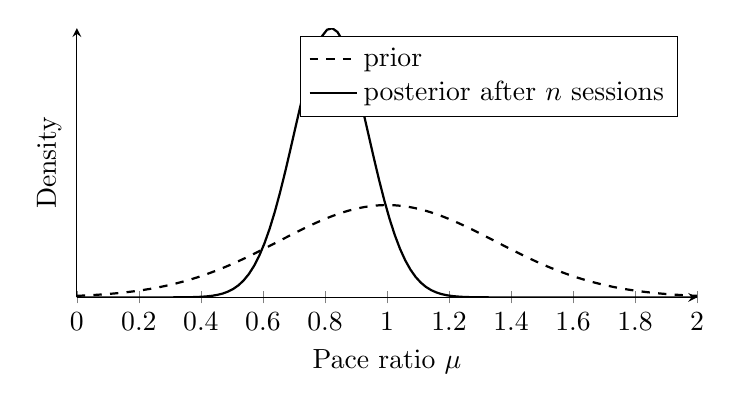
\begin{tikzpicture}
\begin{axis}[width=0.78\linewidth, height=5cm, xlabel={Pace ratio $\mu$}, ylabel={Density}, domain=0:2, samples=120, ymin=0, xmin=0, xmax=2, axis lines=left, ytick=\empty, legend pos=north east, legend cell align=left]
\addplot[thick, dashed]{exp(-(x-1)^2/(2*0.35^2))/(0.35*sqrt(2*pi))};
\addlegendentry{prior}
\addplot[thick]{exp(-(x-0.82)^2/(2*0.12^2))/(0.12*sqrt(2*pi))};
\addlegendentry{posterior after $n$ sessions}
\end{axis}
\end{tikzpicture}
\caption{Schematic illustration of Bayesian pace calibration by Equation~\eqref{eq:bayes-update}: a broad prior over the pace ratio (dashed) tightens to a narrower posterior (solid) as session evidence accumulates. The values shown are illustrative, not measured.}
\label{fig:bayes-update}
\end{figure}

Zanellati et al.~\cite{zanellati2024} review hybrid knowledge-tracing models in a taxonomy of approaches that combine Bayesian posteriors with machine learning, and conclude that hybrid models consistently outperform either pure Bayesian Knowledge Tracing or pure deep learning. Zambrano et al.~\cite{zambrano2024} analyse algorithmic bias in Bayesian Knowledge Tracing at scale and report that performance is essentially equal across demographic groups, which supports the reliable use of Bayesian-family models across diverse learners. Mai et al.~\cite{mai2025} couple deep temporal modelling with a probabilistic layer in a Transformer--Bayesian hybrid that recovers interpretable, calibrated knowledge estimates, reinforcing that a hybrid Bayesian design keeps transparency without sacrificing predictive accuracy. These works establish Bayesian calibration as sound for learner modelling, but they address correctness prediction rather than the planned-versus-actual pace estimation this project requires.

\section{Behavioural-Change Detection}
A learner's pace is not stationary, and detecting when it shifts is what makes timely replanning possible. Saqr et al.~\cite{saqr2026} apply critical-slowing-down indicators in an idiographic analysis of 1.67~million practice attempts from 9{,}401 students and find that 88.2\% of disengaging learners exhibit detectable warning signals beforehand, which is strong evidence that per-learner behavioural shifts are recoverable from trace data. Qiao et al.~\cite{qiao2026} provide a PRISMA systematic review of statistical-process-control methods and document the rationale for CUSUM and EWMA control charts and their machine-learning-enhanced variants, though the reviewed applications target manufacturing rather than education.

The cumulative-sum chart is the detector this project builds on. A one-sided chart tracks the running deviation of the pace signal $x_t$ from its in-control mean $\mu_0$,
\begin{equation}
S_0 = 0, \qquad S_t = \max\!\big(0,\; S_{t-1} + (x_t-\mu_0) - k\big), \qquad \text{alarm if } S_t > h,
\label{eq:cusum}
\end{equation}
where the slack $k$ absorbs ordinary day-to-day variation and $h$ is the decision threshold~\cite{qiao2026}. The statistic stays near zero while the pace is stable and accumulates once a genuine shift occurs, raising an alarm when it crosses $h$, as illustrated in Figure~\ref{fig:cusum}.

\begin{figure}[htbp]
\centering
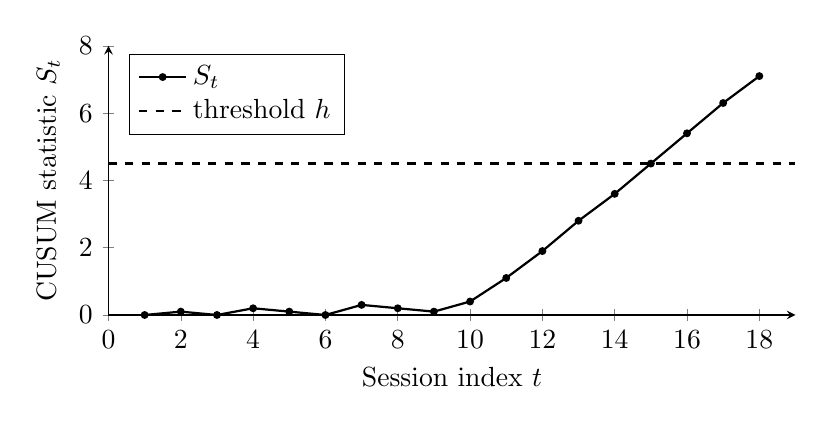
\begin{tikzpicture}
\begin{axis}[width=0.85\linewidth, height=5cm, xlabel={Session index $t$}, ylabel={CUSUM statistic $S_t$}, xmin=0, xmax=19, ymin=0, ymax=8, axis lines=left, legend pos=north west, legend cell align=left]
\addplot[thick, mark=*, mark size=1pt] coordinates {(1,0)(2,0.1)(3,0)(4,0.2)(5,0.1)(6,0)(7,0.3)(8,0.2)(9,0.1)(10,0.4)(11,1.1)(12,1.9)(13,2.8)(14,3.6)(15,4.5)(16,5.4)(17,6.3)(18,7.1)};
\addlegendentry{$S_t$}
\addplot[thick, dashed, domain=0:19]{4.5};
\addlegendentry{threshold $h$}
\end{axis}
\end{tikzpicture}
\caption{Schematic illustration of one-sided CUSUM detection by Equation~\eqref{eq:cusum}: the statistic stays near zero while the pace is stable and accumulates after a shift near $t=10$, raising an alarm when it crosses the threshold $h$. The values shown are illustrative.}
\label{fig:cusum}
\end{figure}

Boca de Giuli et al.~\cite{boca2024} combine control charts with continual learning to separate endogenous system shifts from one-time exogenous disruptions, a distinction that maps directly onto the need to recalibrate on genuine pace change while ignoring a one-off disruption. Cheng et al.~\cite{cheng2024} model behavioural change directly from heterogeneous student records for early at-risk prediction, deliberately retaining qualitative information that pure feature extraction discards. The limitation shared across these methods is that they detect a shift but prescribe no corrective action, which is the step this project adds by feeding the detected shift into replanning.

\section{Progress Prediction with Gaussian Processes}
Projecting a completion date with a calibrated uncertainty band, rather than a single number, is what makes a projection trustworthy. P\'erez-Suay et al.~\cite{perezsuay2024} apply Gaussian-process (GP) regression with an automatic-relevance-determination kernel to learning-management-system logs and achieve a correlation of $R = 0.89$ for predicting student marks, with interpretable feature weighting. Chen and Yao~\cite{chenyao2025} combine black-hole optimisation for feature selection with a weighted GP-regression ensemble, reporting a root-mean-square error of 0.95 and a mean absolute error of 0.81, and show that GP predictions degrade gracefully as data becomes scarce.

A Gaussian process places a prior over progress curves and conditions it on the observed points. For a test time $x_*$ the predictive distribution is Gaussian, with mean and variance
\begin{equation}
\bar{f}_* = \mathbf{k}_*^{\top}(K+\sigma_n^2 I)^{-1}\mathbf{y}, \qquad
\mathbb{V}[f_*] = k(x_*,x_*) - \mathbf{k}_*^{\top}(K+\sigma_n^2 I)^{-1}\mathbf{k}_*,
\label{eq:gp-pred}
\end{equation}
under a squared-exponential kernel with signal variance $\sigma_f^2$ and length scale $\ell$,
\begin{equation}
k(x,x') = \sigma_f^2 \exp\!\Big(-\tfrac{(x-x')^2}{2\ell^2}\Big).
\label{eq:gp-kernel}
\end{equation}
The predictive variance in Equation~\eqref{eq:gp-pred} is what supplies a calibrated band around the projected finish date, rather than a single point, as illustrated in Figure~\ref{fig:gp-burnup}.

\begin{figure}[htbp]
\centering
\begin{tikzpicture}
\begin{axis}[width=0.85\linewidth, height=5.5cm, xlabel={Time (days)}, ylabel={Cumulative progress (\%)}, xmin=0, xmax=60, ymin=0, ymax=112, axis lines=left, legend pos=north west, legend cell align=left]
\addplot[name path=up, draw=none] coordinates {(25,36)(35,63)(45,86)(55,106)(60,112)};
\addplot[name path=lo, draw=none] coordinates {(25,36)(35,48)(45,61)(55,76)(60,84)};
\addplot[gray!20] fill between[of=up and lo];
\addlegendentry{95\% band}
\addplot[thick, mark=*, mark size=1pt] coordinates {(0,0)(5,7)(10,15)(15,20)(20,30)(25,36)};
\addlegendentry{observed}
\addplot[thick, dashed] coordinates {(25,36)(35,55)(45,74)(55,92)(60,100)};
\addlegendentry{GP projection}
\addplot[thick, dotted, domain=0:60]{100};
\end{axis}
\end{tikzpicture}
\caption{Schematic illustration of a Gaussian-process burn-up projection: observed cumulative progress (solid) is extrapolated to completion (dashed) with a 95\% band that widens with the horizon; the dotted line marks 100\% completion. The values shown are illustrative.}
\label{fig:gp-burnup}
\end{figure}

Lin et al.~\cite{lin2024} introduce a latent Kronecker structure to scale GPs for learning-curve prediction, matching Transformer performance while retaining calibrated uncertainty. Beyond regression, Huang and Wang~\cite{huang2025} use Gaussian-process classification with a meta-heuristic hyper-parameter search to predict student performance bands, and Kayande and Kukreja~\cite{kayande2025} report an integrated multi-modal machine-learning framework for engagement and dropout prediction on educational data. These works validate GP methods on educational data, but they apply the model cross-sectionally to a final outcome rather than to the longitudinal burn-up projection, with a running finish-date estimate, that this project needs.

\section{Adaptive Scheduling and Study-Plan Generation}
The system must turn its estimates into a concrete, regenerated schedule. Islam et al.~\cite{islam2024} couple an artificial neural network for grade prediction, at an accuracy of about 0.73, with dynamic programming for optimal schedule allocation, establishing the predict-then-optimize architecture this project takes as its Pillar-A base paper. The two stages are shown in Figure~\ref{fig:predict-optimize}: a predictive model estimates the learner's pace, and an optimizer turns that estimate into a schedule.

\begin{figure}[htbp]
\centering
\begin{tikzpicture}[node distance=6mm and 13mm, box/.style={draw, rounded corners, minimum height=9mm, minimum width=22mm, align=center, font=\small}, >=Latex]
\node[box] (hist) {Session\\history};
\node[box, right=of hist] (predict) {Predict\\(pace)};
\node[box, right=of predict] (opt) {Optimize\\(schedule)};
\node[box, right=of opt] (plan) {Study\\plan};
\draw[->] (hist) -- (predict);
\draw[->] (predict) -- (opt);
\draw[->] (opt) -- (plan);
\end{tikzpicture}
\caption{The predict-then-optimize architecture~\cite{islam2024} this project adopts and extends: a predictive model estimates the learner's pace, and an optimizer turns the estimate into a schedule.}
\label{fig:predict-optimize}
\end{figure}

The optimize step solves a scheduling problem by dynamic programming. Writing $V(t,\rho)$ for the best achievable cost from day $t$ onward with remaining work $\rho$, the schedule follows a recurrence of the form
\begin{equation}
V(t,\rho) = \min_{0 \le a \le c_t}\ \big[\, \ell(a) + V(t+1,\ \rho - a)\,\big],
\label{eq:dp}
\end{equation}
where $a$ is the study time allocated on day $t$, $c_t$ is that day's capacity, and $\ell$ penalises deadline drift~\cite{islam2024}. Fabregar and Amorado~\cite{fabregar2025} generate expert-quality study plans in 0.32~seconds using a greedy algorithm with prerequisite-constraint satisfaction, which demonstrates fast constraint-based, prerequisite-aware scheduling. Pagano et al.~\cite{pagano2026} report a controlled study of 2{,}064 students in which adaptive learning paths produce substantial efficiency gains over static ones, giving both large-scale evidence that adaptation helps and a template for an adaptive-versus-static evaluation design. Liu et al.~\cite{liu2025} integrate a domain knowledge graph with AI-driven sequencing to construct personalised learning paths that respect concept prerequisites. The limitation across these works is that the generated plan is solved once and does not adapt to the pace the learner actually achieves, which is the feedback this project adds.

\section{Self-Regulated-Learning Analytics}
Self-regulated-learning (SRL) analytics grounds the choice of metrics for a planner that reports back to the learner. Alhazbi et al.~\cite{alhazbi2024} review 25 empirical studies on measuring SRL from trace data and find that most validated indicators relate to time-management skills, which grounds this project's use of schedule adherence and regularity as its behavioural metrics. de Barba et al.~\cite{debarba2025} develop and validate an SRL learning-analytics rubric that maps validated SRL scales onto learning-management-system indicators in a scalable, explainable way.

Uzun et al.~\cite{uzun2025} show that a learner's engagement with analytics feedback is associated with both SRL competence and course performance, which motivates the feedback-oriented design of this project's dashboards. Butt et al.~\cite{butt2025} apply a hybrid machine-learning and rough-set model to identify at-risk learners and trigger personalised interventions. These works supply validated, trace-based indicators of self-regulation, but they stop at the feedback step shown in Figure~\ref{fig:srl-loop}, and none feeds the SRL signal back into an adaptive plan.

\begin{figure}[htbp]
\centering
\begin{tikzpicture}[node distance=7mm and 13mm, box/.style={draw, rounded corners, minimum height=8mm, minimum width=25mm, align=center, font=\small}, >=Latex]
\node[box] (trace) {Trace data\\(sessions)};
\node[box, right=of trace] (ind) {SRL\\indicators};
\node[box, right=of ind] (fb) {Feedback\\to learner};
\draw[->] (trace) -- (ind);
\draw[->] (ind) -- (fb);
\draw[->] (fb.south) to[out=-90, in=-90] (trace.south);
\end{tikzpicture}
\caption{The self-regulated-learning analytics loop the reviewed work supports: trace data yields validated indicators that are fed back to the learner. The reviewed systems stop at feedback; this project extends the loop by feeding the signal into replanning.}
\label{fig:srl-loop}
\end{figure}

\section{Methodology for Sourcing the Surveyed Models}
The literature above was assembled through a repeatable screening pipeline rather than by ad-hoc reading, so that the coverage of each theme is defensible. A raw candidate list of 107 Pillar-A digital object identifiers was collected from database and citation searches. Each candidate was enriched with metadata from CrossRef, OpenAlex, and arXiv, and scored against twelve weighted keyword clusters aligned with the project's components, including Bayesian calibration, change-point detection, Gaussian-process regression, adaptive scheduling, and self-regulated learning. The score thresholded each paper into a strong, good, partial, or weak fit.

The score was treated as advisory rather than decisive. Final selection favoured topical coverage across sub-themes over raw score: one representative work was kept per sub-theme, and higher-scoring but redundant papers were dropped, while a lower-scoring paper was retained when it was the best available fit for a specific narrative role. The screening also rejected keyword false positives, where a paper matched a cluster keyword but was topically unrelated. This curation reduced the raw list to the set of works surveyed in this chapter.

\section{Summary of Approaches}
Table~\ref{tab:litsummary} summarizes the approach families across the components with their strengths and the limitations that motivate this work. The recurring pattern is that each technique is strong in isolation but disconnected from the others: none forms a closed loop from realised pace back to the plan.

\begin{table}[htbp]
\centering
\footnotesize
\caption{Summary of Pillar-A approach families, with strengths and limitations for this project.}
\label{tab:litsummary}
\begin{tabular}{p{3.0cm} p{4.2cm} p{4.2cm}}
\toprule
\textbf{Approach family} & \textbf{Strengths} & \textbf{Limitations for this project} \\
\midrule
Bayesian calibration~\cite{chen2024,zanellati2024,zambrano2024,mai2025} & Works with sparse, per-learner data; interpretable; fair across groups & Targets correctness, not planned-versus-actual pace \\
Change-point detection~\cite{saqr2026,qiao2026,boca2024,cheng2024} & Detects behavioural shifts early; well-founded in statistical process control & Detects only; prescribes no corrective replanning \\
Gaussian-process projection~\cite{perezsuay2024,chenyao2025,lin2024,huang2025,kayande2025} & Calibrated uncertainty; degrades gracefully with little data & Applied cross-sectionally, not to longitudinal burn-up \\
Adaptive scheduling~\cite{islam2024,fabregar2025,pagano2026,liu2025} & Fast, prerequisite-aware; adaptation shown to help & Generated plan is static; no feedback from realised pace \\
SRL analytics~\cite{alhazbi2024,debarba2025,uzun2025,butt2025} & Validated trace-based indicators of self-regulation & Measures behaviour; not tied to adaptive replanning \\
\bottomrule
\end{tabular}
\end{table}

The limitations that motivate this project follow from the table. First, calibration, change detection, projection, and scheduling are each studied in isolation, and no reviewed system integrates them into a single connected loop. Second, behavioural monitoring detects shifts but prescribes no corrective replanning, and the scheduling work is static and does not adapt to realised pace. Third, the Gaussian-process work is cross-sectional, so calibrated learning-curve projection is not applied to ongoing self-directed study. Fourth, self-regulated-learning analytics supplies validated indicators but stops at measurement, without feeding the signal back into the plan.

This project addresses these gaps by extending the predict-then-optimize architecture~\cite{islam2024} into an adaptive loop for a single self-directed learner. It combines hierarchical Bayesian pace calibration with a context-aware shrinkage model~\cite{chen2024}, change-point detection of behavioural shifts surfaced as a recalibration prompt~\cite{saqr2026,qiao2026}, Gaussian-process progress projection with a calibrated uncertainty band~\cite{perezsuay2024}, and capacity-based schedule regeneration~\cite{fabregar2025}, evaluated with the adaptive-versus-static paradigm~\cite{pagano2026} and self-regulated-learning metrics~\cite{alhazbi2024}. Phase~II will extend this open-loop system with assessment-based verification of genuine learning, so that the pace signal driving the plan is checked against evidence of learning rather than self-reported time alone.
